%\documentclass[dvipdfmx]{beamer}
\documentclass[dvipdfmx,final,t,12pt]{beamer}
\usepackage[orientation=portrait,size=a4,scale=1.4]{beamerposter}%縦 : orientation=portrait, 横 : orientation=landscape
\usepackage{here, amsmath, latexsym, amssymb, bm, ascmac, mathtools, multicol, tcolorbox}
\usepackage{listings}
%\usepackage{luatexja}
%\usepackage{luatexja-otf}
%\usepackage[match]{luatexja-fontspec}
%\usepackage[]{luatexja-preset}

%\AtBeginDvi{\special{pdf:mapfile ptex-ipa.map}}

\renewcommand{\kanjifamilydefault}{\gtdefault}
\usepackage[deluxe, expert]{otf}
\usepackage{minijs}  %min10

\lstset{
    frame=single,
    basicstyle={\ttfamily\footnotesize},
}

%カラーテーマの選択(省略可)
%\usecolortheme{orchid}
\usetheme{zurichposter}
%フォントテーマの選択(省略可)
\usefonttheme{professionalfonts}
%フレーム内のテーマの選択(省略可)
\useinnertheme{circles}

%ナビゲーションバー非表示
\setbeamertemplate{navigation symbols}{}
%既定をゴシック体に
\renewcommand{\kanjifamilydefault}{\gtdefault}
%itemize
%\setbeamertemplate{itemize item}{\small\raise0.5pt\hbox{$\bullet$}}
%\setbeamertemplate{itemize subitem}{\tiny\raise1.5pt\hbox{$\blacktriangleright$}}
%\setbeamertemplate{itemize subsubitem}{\tiny\raise1.5pt\hbox{$\bigstar$}}
% color
%\newcommand{\red}[1]{\textcolor{red}{#1}}
%\newcommand{\green}[1]{\textcolor{green!40!black}{#1}}
%\newcommand{\blue}[1]{\textcolor{blue!80!black}{#1}}
%head
%\setbeamertemplate{headline}{
%    \begin{center}
%        \structure{
%            \vskip3ex
%            \rule{0.98\linewidth}{4mm}
%            \vskip3ex
%            \usebeamercolor{title in headline}{\textbf{\LARGE{\inserttitle}}\\[2.5ex]}
%            \usebeamercolor{author in headline}{\large{\insertauthor}\\[1.2ex]}
%            \usebeamercolor{institute in headline}{\large{\insertinstitute}}
%            \vskip3ex
%            \rule{0.98\linewidth}{4mm}
%        }
%    \end{center}
%}


\setbeamerfont{block title}{size=\Large}
\setbeamerfont{block body}{size=\large}

\setbeamertemplate{itemize/enumerate body begin}{\large}
\setbeamertemplate{itemize/enumerate subbody begin}{\large}

%\setbeamersize{text margin left = 2.5ex, text margin right = 1.2ex}
%\addtobeamertemplate{block begin}{\ }{}
%\setbeamercolor{block body}{bg=gray}

\title{組込みシステム向けFRP言語の\\静的スケジューリングを用いた並列化}
\author{櫻井義孝・渡部卓雄}
\institute{東京工業大学}


\begin{document}

\begin{frame}[fragile]
    \begin{block}{概要}
        \vskip 1ex
        \begin{itemize}
            \item 目的:小規模組込みシステム向けFRP言語の応答性向上
            \item 既存の小規模組込みシステム向けFRP言語であるEmfrpはシングルスレッドで動作する
                \begin{itemize}
                    \item マルチスレッドが使用可能な環境では計算資源を十分に活用できない
                \end{itemize}
            \item 本研究では応答性向上のために静的スケジューリングを用いてEmfrpを並列化することを提案する
        \end{itemize}
        \vskip -2.5ex
    \end{block}

    \begin{block}{Emfrp \small{[Sawada2016]}}
        \begin{columns}
            \begin{column}{0.45\textwidth}
                \vskip -1.15ex
                小規模組込みシステム向けFRP言語
                \lstinputlisting{./code/FanController.xfrp}
                \begin{center}
                    \vskip -3ex
                    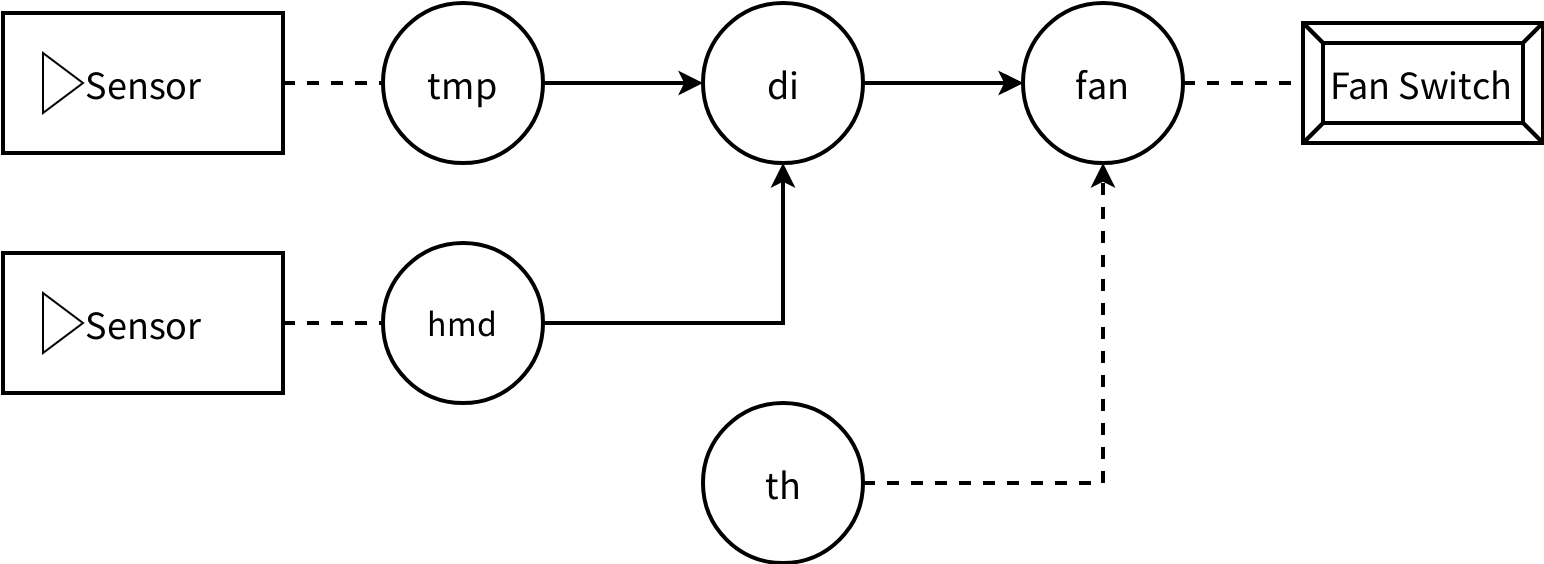
\includegraphics[scale=0.15]{./image/FanController.png}
                \end{center}
            \end{column}
            \begin{column}{0.45\textwidth}
                \begin{itemize}
                    \item 時変値をノードとし依存関係を辺とした有向非巡回グラフ(DAG)を構成
                    \item Emfrpの処理系では依存関係に沿ってノードの値を順次更新することを繰り返しりアクティブなシステムを実現している
                    \item この例では例えばtmp$\rightarrow$hmd$\rightarrow$di$\rightarrow$th$\rightarrow$fanの順
                    \item しかし,現在のEmfrpの処理系はノードの更新が逐次的に行われているので,ノードの更新を並列に行うことを提案する
                    \item OSがない環境や小規模なFree-RTOSなどの環境ではOSによるスケジューリングが利用できないことがある
                    \item またOSのスケジューリングが可能な場合でも
                    \item そこでそのような環境にも対応するため静的にスケジューリングすることを提案する
                    %\item { TODO: 組込みシステムでは普通のコンピュータとどの辺りが異なるかとかなぜ静的に並列化するかとか}
                \end{itemize}
            \end{column}
        \end{columns}
    \end{block}

    \begin{block}{並列化アルゴリズム}
        \begin{columns}
            \begin{column}{0.6\textwidth}
                \begin{enumerate}
                    \item 各ノードからsinkノードへの最長距離を計算
                    \item TODO: sinkノードの説明(図にどれがsinkノードなのかの説明を入れる)
                    \item 同じ距離にあるノードを並列に実行
                        \begin{itemize}
                            %\item 必要な場合は同時実行できるノードの数をスレッド数で割った数のノードを1スレッドが処理する
                            \item OSのスケジューラーを利用できない環境ではどのプロセッサがどのノードを処理するかを指定する必要があるのでその説明を行う
                        \end{itemize}
                \end{enumerate}

                \begin{table}[c]
                    \begin{tabular}{|c|c|c|c|}
                        \hline
                        出力ノードまでの距離 & 2   & 1     & 0                                                    \\ \hline
                        同時に処理するノード & 0,4 & 1,2,6 & \begin{tabular}[c]{@{}l@{}}3,5,\\ 7,8,9\end{tabular} \\ \hline
                    \end{tabular}
                \end{table}
            \end{column}
            \begin{column}{0.3\textwidth}
                \begin{center}
                    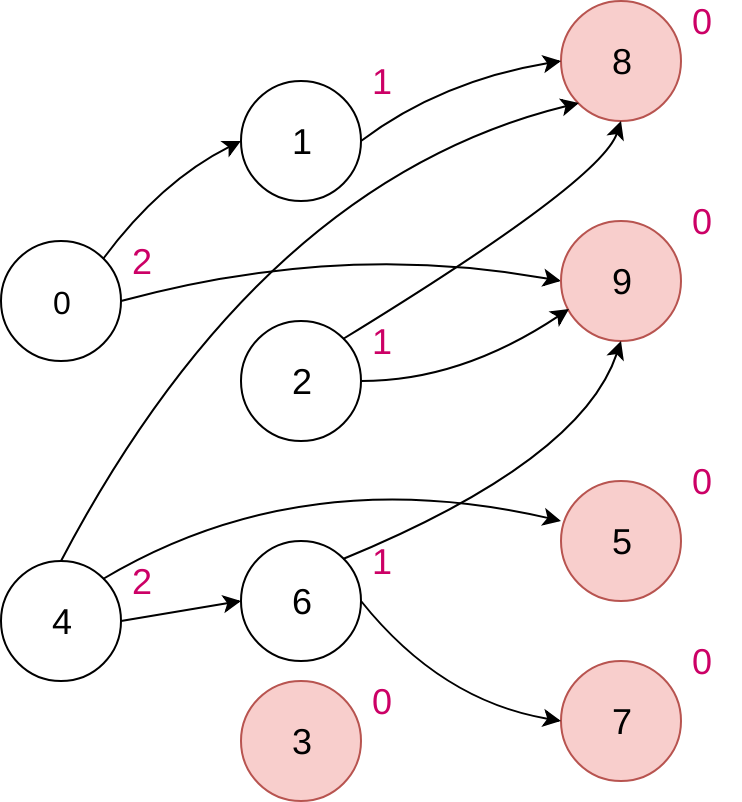
\includegraphics[scale=0.2]{image/RandomGraph.png}
                \end{center}
            \end{column}
        \end{columns}
    \end{block}

    \begin{block}{実験}
        \begin{itemize}
            \item 環境
            \item 対象アプリケーション : ライフゲーム
        \end{itemize}
    \end{block}
\end{frame}
\end{document}
